%% Slides that accompany the research proposal in ../../proposal/.
%% Theme: the Pradita beamer theme in ../theme/, copied from the slides of the
%% course Advanced Web Engineering. The theme loads fontspec, so the deck builds
%% with XeLaTeX:  latexmk -xelatex talk.tex
%% Writing rules of the project: plain words, no overclaiming, short sentences,
%% no pronouns and no em or en dashes.
\documentclass[aspectratio=169, table, 12pt]{beamer}

\usepackage{colortbl}
\usepackage{xcolor}
\usepackage{tabularx}
\usepackage{booktabs}
\usepackage{tikz}
\usetikzlibrary{arrows.meta, positioning, calc}

\makeatletter
\def\input@path{{../theme/}}
\makeatother
\graphicspath{{../theme/}{../../proposal/figures/}{../../../../papers/01-SoSym/paper/figures/}}
\usetheme{Pradita}

%% The theme defines praditagreen as the green of the university logo (#0E6333).

%% The theme draws table rules in white. Black rules keep the tables readable.
\arrayrulecolor{black}
\setlength{\arrayrulewidth}{0.5pt}

%% Left-aligned X column, so narrow table cells keep normal word spacing.
\newcolumntype{Y}{>{\raggedright\arraybackslash}X}

\title{\Huge Towards Decentralized\\ \vspace{10pt} Model Persistence}
\subtitle{Research proposal}
\author{\textbf{Alfa Yohannis}}
\date{September 2026}

\begin{document}

\frame{\titlepage}

\begin{frame}
  \frametitle{Outline}
  \vspace{20pt}
  \begin{columns}[t]
    \column{0.5\textwidth}
    \tableofcontents[sections={1-3}]
    \column{0.5\textwidth}
    \tableofcontents[sections={4-5}]
  \end{columns}
\end{frame}

\begin{frame}{\hfill}
  \centering
  \huge{\textbf{Can engineering models\\[6pt] be developed in a\\[6pt] decentralized, immutable way?}}\\[22pt]
  \large Today a model refers to another model by a file name,\\
  and the file can change under the reference.
\end{frame}

%% ---------------------------------------------------------------------------
\section{Problem}

\begin{frame}{\hfill}
  \centering
  \Huge{\textbf{Problem}}
\end{frame}

\begin{frame}{{\Large Addresses Name Locations}}
  \vspace{10pt}
  \begin{itemize}
    \item The Eclipse Modeling Framework (EMF) keeps each model in a resource,
          and a Uniform Resource Identifier (URI) names the resource.
    \item Common URIs such as \texttt{file://} and \texttt{platform://} name a
          location, and the content at the location can change.
    \item A reference therefore resolves to whatever the location holds at the
          moment of the read.
    \item The InterPlanetary File System (IPFS) names content by a content
          identifier (CID), computed from the content itself.
  \end{itemize}
  \vspace{8pt}
  {\footnotesize A changed model receives a new CID, so a reference by CID keeps
  pointing at the version that was referenced.}
\end{frame}

\begin{frame}{{\Large Local and Decentralized Development}}
  \vspace{14pt}
  \centering
  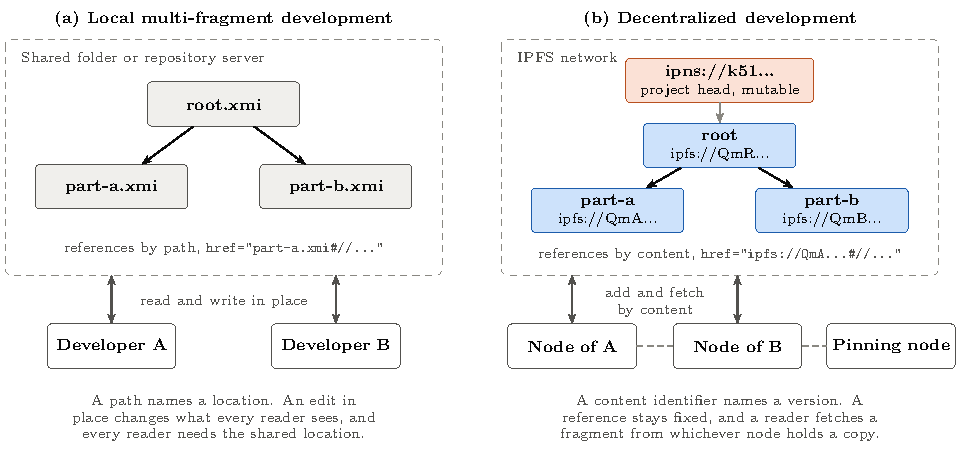
\includegraphics[height=0.7\textheight]{development-settings.pdf}
\end{frame}

\begin{frame}{{\Large Where the Gap Hurts}}
  \vspace{10pt}
  \begin{itemize}
    \item A team shares one metamodel. An edit to the shared file changes the
          meaning of every referring model, and no reference records the
          intended version.
    \item Reverse engineering produces a snapshot of a code base, yet a file
          path does not name a snapshot.
    \item Partners exchange models across organizations, and a path inside one
          organization means nothing inside another.
  \end{itemize}
  \vspace{8pt}
  {\footnotesize A reference that names a version would remove the ambiguity in
  all three settings.}
\end{frame}

\begin{frame}{{\Large Two Kinds of Address}}
  \vspace{14pt}
  \centering
  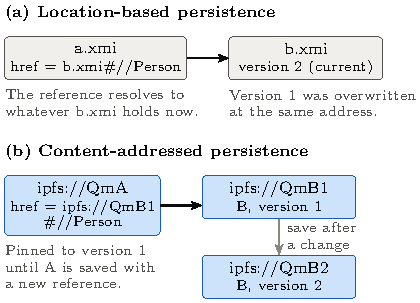
\includegraphics[height=0.66\textheight]{version-pinning.pdf}
\end{frame}

%% ---------------------------------------------------------------------------
\section{State of the Art}

\begin{frame}{\hfill}
  \centering
  \Huge{\textbf{State of the Art}}
\end{frame}

\begin{frame}{{\Large What Exists and What Is Missing}}
  \vspace{8pt}
  \begin{itemize}
    \item Scalable persistence, for example Morsa, NeoEMF, CDO and Hawk, keeps
          identifiers stable inside a store while the content changes.
    \item Versioning and comparison, for example EMFStore and EMF Compare,
          record or compute what changed between two states.
    \item Content addressing outside modeling, for example Venti, Git, Nix,
          Software Heritage and IPFS, gives addresses that never change.
  \end{itemize}
  \vspace{10pt}
  \begin{tcolorbox}[colback=praditagreen!8, colframe=praditagreen, boxrule=0.6pt, arc=2pt]
    \small No reviewed approach stores EMF models under content identifiers,
    and none describes references between resources whose identifiers change
    on every save.
  \end{tcolorbox}
\end{frame}

%% ---------------------------------------------------------------------------
\section{Research Questions}

\begin{frame}{\hfill}
  \centering
  \Huge{\textbf{Research Questions}}
\end{frame}

\begin{frame}{{\Large Three Questions}}
  \vspace{16pt}
  \small
  \begin{description}[RQ3]
    \item[RQ1] \textbf{Architecture.} Which challenges arise when a model
          persistence framework stores models by content, and how can the
          challenges be addressed?\\
          {\footnotesize URI handling, a resource without an identifier before
          the first save, and file resources next to IPFS resources.}
    \item[RQ2] \textbf{Cross-resource references.} How do references survive
          when every save gives a resource a new identifier?\\
          {\footnotesize Reference strategies, the update of referencing
          resources, cycles, and models split into many resources.}
    \item[RQ3] \textbf{Performance.} What does content-addressed persistence
          cost, and when is the cost acceptable?\\
          {\footnotesize Save and load times against local files, from small
          models to several hundred thousand elements.}
  \end{description}
\end{frame}

%% ---------------------------------------------------------------------------
\section{Method and Plan}

\begin{frame}{\hfill}
  \centering
  \Huge{\textbf{Method and Plan}}
\end{frame}

\begin{frame}{{\Large Research Design}}
  \vspace{16pt}
  \centering
  
\includegraphics[width=\textwidth]{research-design.pdf}\\[10pt]
  {\footnotesize The study follows design science (Hevner et al., 2004), and
  the case study follows the guidelines of Runeson and H\"ost (2009).}
\end{frame}

\begin{frame}{{\Large Planned Persistence Layer}}
  \vspace{14pt}
  \centering
  
\includegraphics[height=0.68\textheight]{planned-layer.pdf}
\end{frame}

\begin{frame}{{\Large Work Plan}}
  \vspace{12pt}
  \centering
  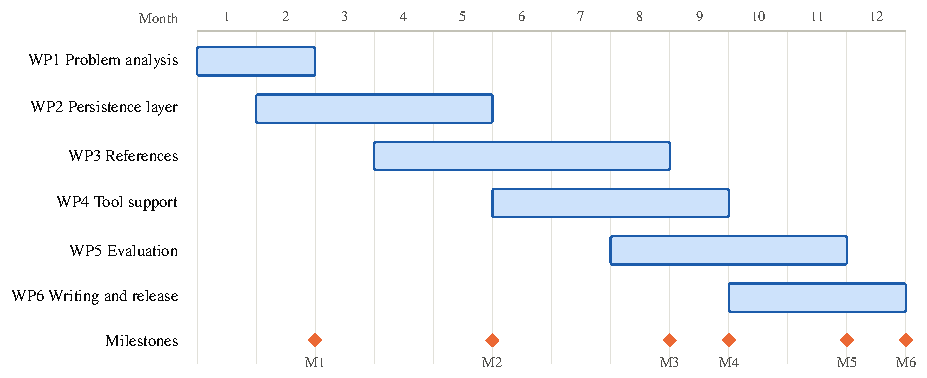
\includegraphics[width=\textwidth]{work-plan.pdf}\\[6pt]
  {\footnotesize Six months, six work packages and five milestones, from the
  problem analysis to a submitted manuscript with a public artifact.}
\end{frame}

\begin{frame}{{\Large Evaluation Plan}}
  \vspace{10pt}
  \begin{columns}[t]
    \column{0.32\textwidth}
    \textbf{Functional validation}\\[4pt]
    {\small Tests and example programs for round trips, mixed resource sets,
    references across resources and proxy resolution.}
    \column{0.32\textwidth}
    \textbf{Benchmark}\\[4pt]
    {\small Generated models from 100 to several hundred thousand elements,
    thirty measured runs per size and a paired statistical test.}
    \column{0.32\textwidth}
    \textbf{Case study}\\[4pt]
    {\small About one gigabyte of MoDisco models of the Eclipse Java
    development tools, published on IPFS and fetched back for comparison.}
  \end{columns}
\end{frame}

%% ---------------------------------------------------------------------------
\section{Outcomes and Resources}

\begin{frame}{\hfill}
  \centering
  \Huge{\textbf{Outcomes and Resources}}
\end{frame}

\begin{frame}{{\Large Contributions and Deliverables}}
  \vspace{8pt}
  \begin{itemize}
    \item An EMF resource implementation that saves models on IPFS and loads
          models by CID or by a mutable IPNS name.
    \item Strategies for references between content-addressed resources,
          with an algorithm that updates referencing resources after a change.
    \item IPFS support inside the Eclipse BPMN2 Modeler and a generated tree
          editor.
    \item An evaluation on generated models and on large reverse-engineered
          models.
  \end{itemize}
  \vspace{6pt}
  {\footnotesize Deliverables: public repositories, evaluation scripts and
  results, a dataset archived under a DOI, and a manuscript for Software and
  Systems Modeling (SoSyM).}
\end{frame}

\begin{frame}{{\Large Risks and Mitigation}}
  \vspace{14pt}
  {\centering\footnotesize
  \begin{tabularx}{\textwidth}{@{}YY@{}}
    \toprule
    \textbf{Risk} & \textbf{Mitigation} \\
    \midrule
    The resource model of EMF resists a changing identifier &
      Early proof of concept, with a placeholder address before the first save \\
    A reference cycle cannot settle under immutable identifiers &
      Detect cycles before publication, and report the limit \\
    The update of referencing resources grows expensive on a large graph &
      Measure on the case study model, and compare a scan with a manifest index \\
    Measurements vary with the machine and the node &
      Fixed heap, warm-up runs, an idle machine, an offline node and a paired test \\
    A published model becomes unavailable &
      Pin the content on a project node, and archive the dataset under a DOI \\
    \bottomrule
  \end{tabularx}\par}
\end{frame}

\begin{frame}{{\Large Budget}}
  \vspace{13pt}
  {\centering\footnotesize
  \renewcommand{\arraystretch}{1.05}
  \begin{tabular}{@{}lrr@{}}
    \toprule
    \textbf{Category} & \textbf{USD} & \textbf{IDR} \\
    \midrule
    Researcher, 6 months at IDR 2,000,000 & 706 & 12,000,000 \\
    Assistant, 6 months at IDR 2,000,000 & 706 & 12,000,000 \\
    Storage and pinning & 250 & 4,250,000 \\
    Two domain names at Cloudflare & 22 & 374,000 \\
    Archiving on Zenodo & 0 & 0 \\
    Flight to a conference in Japan or Korea & 600 & 10,200,000 \\
    Accommodation, four nights & 360 & 6,120,000 \\
    Conference registration & 600 & 10,200,000 \\
    Meals and local transport, five days & 250 & 4,250,000 \\
    \midrule
    \textbf{Subtotal} & \textbf{3,494} & \textbf{59,394,000} \\
    Open access fee of the journal, optional & 3,190 & 54,230,000 \\
    \textbf{Total} & \textbf{6,684} & \textbf{113,624,000} \\
    \bottomrule
  \end{tabular}\par}
  \vspace{4pt}
  {\tiny\centering Estimates at IDR 17,000 per USD. The journal fee applies only
  to the open access route.\par}
\end{frame}

\begin{frame}{\hfill}
  \centering
  \Huge{\textbf{Thank you}}\\[18pt]
  \normalsize Alfa Yohannis, Department of Informatics, Pradita University\\[4pt]
  \href{mailto:alfa.ryano@pradita.ac.id}{alfa.ryano@pradita.ac.id}\\[10pt]
  \small Target venue:
  \href{https://link.springer.com/journal/10270}{Software and Systems Modeling (SoSyM)}
\end{frame}

\end{document}
